\input{myarticlepreamble}
\input{yliow}
\renewcommand\TITLE{latextool}

\usetikzlibrary{shapes.geometric}

\begin{document}
\topmatter


\newpage\myinput{notes.tex}
\newpage\myinput{testmylist.tex}
\newpage\myinput{execute.tex}
\newpage\myinput{console.tex}
\newpage\myinput{python.tex}
\newpage\myinput{verbatim.tex}
\newpage\myinput{textcolor.tex}
\newpage\myinput{table.tex}

\newpage\myinput{plot.tex}
\newpage\myinput{grid.tex}

\newpage\myinput{tabrect.tex}

\newpage\myinput{scaling.tex}
\newpage\myinput{line.tex}
\newpage\myinput{circle.tex}

\newpage\myinput{rect.tex}

\newpage\myinput{array.tex}

\newpage\myinput{rectcontainer.tex}
\newpage\myinput{snipped-array.tex}

\newpage\myinput{singlylinkedlist.tex}

\newpage\myinput{doublylinkedlist.tex}
\newpage\myinput{position.tex}
\newpage\myinput{tree.tex}
\newpage\myinput{tree2.tex}

\newpage\myinput{graph.tex}

\newpage\myinput{chunkedarray.tex}
\newpage\myinput{array2d.tex}
\newpage\myinput{bend.tex}
\newpage\myinput{arc.tex}
\newpage\myinput{shell.tex}

\newpage\myinput{frame.tex}
\newpage\myinput{test-verbatim-spacing.tex}

\newpage\myinput{automata.tex}

\newpage\myinput{vec2d.tex}

\newpage\myinput{line-graph.tex}


\newpage
\section{TEST ISOCELES TRIANGLE}


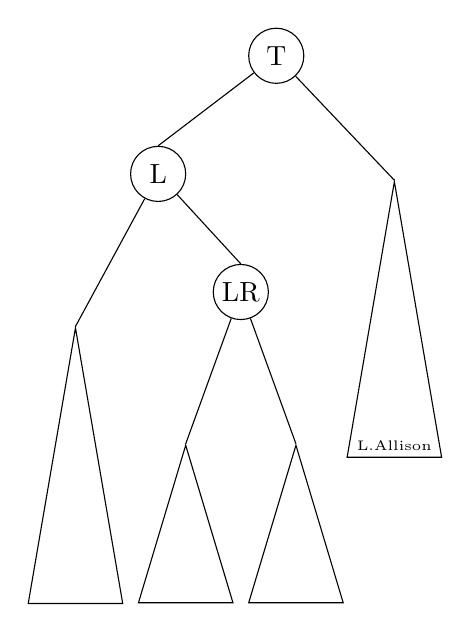
\begin{tikzpicture}[
  inner/.style={circle,draw,minimum width=7mm,inner sep=0},
  leaf/.style={isosceles triangle,draw,shape border rotate=90,isosceles triangle stretches=true, minimum height=20mm,minimum width=12mm,inner sep=0,yshift={-20mm},font=\tiny},
  large leaf/.style={leaf,minimum height=35mm,yshift={-14.5mm}},
  level 1/.style={sibling distance=30mm},
  level 2/.style={sibling distance=21mm},
  level 3/.style={sibling distance=14mm},
]
  \node[inner] {T}
    [child anchor=north]
    child {node[inner] {L}
      child {node[large leaf] {}}
      child {node[inner] {LR}
        child{node[leaf] {}}
        child{node[leaf] {}}}}
    child {node[large leaf] {L.Allison}};
\end{tikzpicture}

\verb!http://tex.stackexchange.com/questions/7862/triangle-node-with-adjustable-height!

\verb!http://tex.stackexchange.com/questions/37462/placing-a-triangle-around-nodes-in-a-tree!

\end{document}
